\documentclass[fr]{../../../../../../eplexam}
\usepackage{../../../../../../eplchem}
\usepackage{../../../../../../eplunits}

\newcommand{\estd}[1]{E\std_{\text{#1}}}
\newcommand{\ecell}{\estd{cell}}
\newcommand{\eca}{\estd{cathode}}
\newcommand{\ean}{\estd{anode}}
\DeclareSIUnit\molar{\textsc{m}}
\newcommand*\diff{\mathop{}\!\mathrm{d}} % Differential operator
\newcommand{\Ea}{E_{\text{a}}} % Direct activation energy
\newcommand{\Eaa}{E_{\text{a}}'} % Inverse activation energy
\newcommand{\deltr}[1]{\Delta_{\text{#1}}} % Transformation delta
\usepackage{breqn} % Needed for using \left and \right in long equations
\usepackage{physics}

\hypertitle{Chimie et chimie physique}{3}{FSAB}{1302}{2014}{Janvier}{All}
{Martin Braquet \and Gilles Peiffer}
{Hervé Jeanmart, Christian Bailly et Francis Delannay}

\section{( /10)}

Soit la réaction élémentaire équilibrée $\ce{A <=> B}$. Supposons que le système soit à l’équilibre à
une température $T_1$ de départ et qu’on le porte très brutalement (= instantanément) à une
température finale $T_2$.
\begin{enumerate}
    \item dans quels cas, le système est-il encore à l’équilibre immédiatement après le saut de
température et dans quels cas ne l’est-il plus? Expliquez brièvement votre réponse.
\item dans le cas où le système n’est plus à l’équilibre immédiatement après le saut, trouvez les
équations cinétiques différentielle et intégrée du retour à l’équilibre. \textit{Suggestion : utilisez
l’écart aux concentrations d’équilibre comme variable dans les équations pour les simplifier.}
\end{enumerate}

\begin{solution}

\begin{enumerate}
    \item Dans le cas d'une réaction réversible rapide, le système adapte instantanément les concentrations des composés pour satisfaire la constante d'équilibre.
    \item
    Soit
    \begin{itemize}
        \item $k_1$: la constante de vitesse de la réaction directe à la température $T_1$;
        \item $k_1'$: la constante de vitesse de la réaction inverse à la température $T_1$;
        \item $k_2$: la constante de vitesse de la réaction directe à la température $T_2$;
        \item $k_2'$: la constante de vitesse de la réaction inverse à la température $T_2$.
    \end{itemize}
    On a, après le saut et donc à la température $T_2$:
    $$\phantom{.} \dv{\ce{[A]}}{t}= -k_2\ce{[A]}+k_2'\ce{[B]}.$$
    Puisque $\ce{[A] + [B]} = \text{Cst}=\ce{[A]}_0 + \ce{[B]}_0$ (avec $\ce{[A]}_0$ et $\ce{[B]}_0$ les concentrations au moment du saut, et aussi les concentrations d'équilibre à $T_1$),
    \begin{align*}
     \dv{\ce{[A]}}{t} &= -k_2\ce{[A]} + k_2'(\ce{[A]}_0 + \ce{[B]}_0 - \ce{[A]})\\
    				  &= -(k_2+k_2')\ce{[A]} + k_2'(\ce{[A]}_0 + \ce{[B]}_0).
     \end{align*}
    Cette EDO ne doit plus être manipulée car l'unique inconnue est $\ce{[A]}$ et les autres termes sont des constantes indépendantes de $\ce{[A]}$.
    On la résout ensuite:
     \begin{equation*}
          \int^{\ce{[A]}}_{\ce{[A]}_0}\frac{\diff{\ce{[A]}}}{(k_2+k_2')\ce{[A]}-k_2'(\ce{[A]}_0+\ce{[B]}_0)} = -\int_0^t\diff{\tau}
     \end{equation*}
     \begin{equation*}
          \frac{1}{(k_2+k_2')} \ln \frac{(k_2+k_2') \ce{[A]}-k_2'(\ce{[A]}_0 + \ce{[B]}_0)}{(k_2+k_2') \ce{[A]}_0-k_2'(\ce{[A]}_0 + \ce{[B]}_0}) = -t
     \end{equation*}
     \begin{equation*}
          \phantom{.} \ce{[A]} = \frac{1}{(k_2+k_2')} \left(\left(k_2\ce{[A]}_0 - k_2' \ce{[B]}_0\right) \e^{\left(-(k_2+k_2')t\right)} + k_2'(\ce{[A]}_0+\ce{[B]}_0)\right).
     \end{equation*}
     Puisqu'on ne connaît a priori pas les constantes de vitesse à la température $T_2$, on peut les exprimer en fonction de celles à $T_1$ en utilisant
     \begin{equation*}
          \phantom{.} k_2 = k_1 \exp \left(\frac{\Ea}{R} \left(\frac{1}{T_1} - \frac{1}{T_2}\right) \right).
     \end{equation*}
     On a finalement
     \begin{dmath*}
               \phantom{,} \ce{[A]}_t = \frac{1}{\left(k_1 \exp(\Ea) + k_1' \exp(\Eaa) \right)} \left( k_1' \exp(\Eaa)(\ce{[A]}_0 + \ce{[B]}_0) + \left(k_1 \exp(\Ea) \ce{[A]}_0 - k_1' \exp(\Eaa) \ce{[B]}_0\right)
               \e^{\left( -\exp \left(\frac{1}{R} \left(\frac{1}{T_1} - \frac{1}{T_2}\right) \right) \left(k_1 \exp(\Ea) + k_1' \exp(\Eaa) \right) t \right)}\right),
     \end{dmath*}

     avec $\Ea$ et $\Eaa$ les énergies d'activation des réactions directe et inverse.

     Puisque $k_1 \ce{[A]}_0 = k_1' \ce{[B]}_0$ :

     \begin{dmath*}
               \phantom{.} \ce{[A]}_t = \frac{1}{\left(k_1 \exp(\Ea) + k_1' \exp(\Eaa)\right)} \left(k_1' \exp(\Eaa) (\ce{[A]}_0 + \ce{[B]}_0) + k_1 \ce{[A]}_0
               \e^{\left(-\exp \left(\frac{1}{R}\left(\frac{1}{T_1} - \frac{1}{T_2}\right)\right) \left(k_1 \exp(\Ea) + k_1' \exp(\Eaa)\right)(\Ea - \Eaa) t \right)}\right).
     \end{dmath*}

     Une vérification est toujours intéressante.

     Au temps initial, on a :
     \begin{equation*}
          \begin{split}
               \ce{[A]}(0) &= \frac{\left(k_1'\exp(\Eaa)(\ce{[A]}_0 + \ce{[B]}_0) + (k_1\exp(\Ea)\ce{[A]}_0 - k_1' \exp(\Eaa)\ce{[B]}_0)\right)}{(k_1 \exp(\Ea) + k_1' \exp(\Eaa))} \\
               &= \frac{1}{(k_1 \exp(\Ea) + k_1' \exp(\Eaa))} \left(k_1' \exp(\Eaa)\ce{[A]}_0 + k_1 \exp(\Ea) \ce{[A]}_0\right) \\
               &= \ce{[A]}_0.
          \end{split}
     \end{equation*}

     De plus, au nouvel équilibre à $T_2$,

     \begin{equation*}
          \begin{split}
               \ce{[A]}(t \to \infty) &= \frac{k_1' \exp(\Eaa)(\ce{[A]}_0 + \ce{[B]}_0)}{(k_1 \exp(\Ea) + k_1' \exp(\Eaa))} \\
               &= \frac{k_2' (\ce{[A]}_\infty+\ce{[B]}_\infty)}{(k_2 + k_2')} \\
               &= \frac{k_2' \ce{[A]}_\infty + k_2 \ce{[A]}_\infty}{(k_2 + k_2')} \\
               &= \ce{[A]}_\infty,
          \end{split}
     \end{equation*}
     puisqu'à l'équilibre, $k_2 \ce{[A]} = k_2'\ce{[B]}$.

     Pour terminer, supposons que la température augmente et que la réaction soit endothermique ($\Ea > \Eaa$). L'argument de l'exponentielle est négatif, la fonction est dès lors décroissante puisque tous les autres termes sont positifs. On voit donc bien que la concentration du réactif diminue comme le veut le principe de Le Chatelier.

\end{enumerate}

\end{solution}

\section{( /5)}

Soit l’équation globale $\ce{A + B -> C}$.

On ne connaît a priori rien du mécanisme. Pour établir les
ordres de réaction, une analyse de "dégénérescence d’ordre"  est effectuée.
Qu’est ce que la dégénérescence d’ordre ?

Si elle a mis en évidence un ordre partiel $0$ pour le réactif B, quelle conclusion logique peut-on en tirer sur le mécanisme de réaction ?

\begin{solution}

La dégénérescence caractérise le fait que la vitesse de réaction est indépendante de la concentration d'un des réactifs. Elle apparaît lorsque la concentration de ce réactif est nettement supérieure à la concentration des autres réactifs. Cette technique permet d'analyser la vitesse de réaction en fonction d'un réactif cible dont la concentration est très faible par rapport à celle des autres réactifs.

On peut conclure que cette réaction est issue de deux réactions élémentaires :
\begin{itemize}
    \item $\ce{A -> D}$ ou $\ce{2A -> 2D}$  (lente)
    \item $\ce{D + B -> C}$ (rapide)
\end{itemize}
La réaction globale sera donc d'ordre 1 ou 2 par rapport à $\ce{A}$ suivant le mécanisme de la première réaction élémentaire.

\end{solution}

\section{( /5)}
Dans la réaction de craquage thermique de l’éthane, le mécanisme réactionnel, comme vu au cours, est le suivant :

\begin{enumerate}
    \item $\ce{CH3 - CH3 -> CH3^{.} + CH3^{.}}$ (lent)
    \item $\ce{CH3^{.} + CH3-CH3 -> CH4 + CH3-CH2^{.}}$ (rapide)
    \item $\ce{CH3-CH2^{.} -> CH2=CH2 + H^{.}}$
    \item $\ce{CH3-CH3 + H^{.} -> CH3-CH2^{.} + H2}$
    \item $\ce{CH3-CH2^{.} + CH3-CH2^{.} -> CH3-CH2-CH2-CH3}$
\end{enumerate}
Expliquez et utilisez l’hypothèse de stationnarité des radicaux pour calculer la concentration stationnaire des radicaux $\ce{CH3-CH2^{.}}$ en fonction de celle en réactif $\ce{CH3-CH3}$.

\begin{solution}

Les explications sont dans les slides de la partie \textit{cinétique chimique}. Voici néanmoins une brève réponse:

Les réactions de propagation (c-à-d, les réactions 1 et 2) se passent à la même vitesse et n'interviennent donc pas dans les vitesses d'apparition et de disparition de $\ce{CH3-CH2^{.}}$.

On a donc:
\begin{equation*}
     \phantom{.} r_{\ce{CH3-CH2^{.}}\text{,prod}} = 2k_{\text{init}}\ce{[CH3-CH3]} \qquad \text{et} \qquad r_{\ce{CH3-CH2^{.}}\text{,disp}} = 2k_{\text{term}} \ce{[CH3-CH2^{.}]}^2.
\end{equation*}

Par hypothèse de quasi-stationnarité des radicaux, les vitesses d'apparition et de disparition des radicaux sont identiques, et on a donc que
\begin{equation*}
     \phantom{.} r_{\ce{CH3-CH2^{.}}\text{,prod}} = r_{\ce{CH3-CH2^{.}}\text{,disp}}.
\end{equation*}

En exprimant en fonction des concentrations, on trouve alors

\begin{equation*}
     \begin{split}
          2k_{\text{init}} \ce{[CH3-CH3]} &= 2k_{\text{term}} \ce{[CH3-CH2^{.}]}^2 \\
          \implies \qquad \ce{[CH3-CH2^{.}]} &= \left(\frac{k_{\text{init}}}{k_{\text{term}}}\right)^{1/2} \ce{[CH3-CH3]}^{1/2}.
     \end{split}
\end{equation*}

\end{solution}

\section{( /7)}

La fraction molaire de $\ce{O2}$ dans l’atmosphère terrestre est égale à $\SI{0.2}{\mol \per \litre}$. Étant donné les deux états de
valence possibles du fer, il existe plusieurs oxydes de fer différents. Nous ne considérons ici que le
$\ce{FeO}$ et le $\ce{Fe2O3}$, qui peuvent se former dans l’atmosphère via les réactions
\begin{equation}
     \ce{Fe + (1/2) O2 -> FeO}
\end{equation}
ou
\begin{equation}
     \ce{2Fe + (3/2) O2 -> Fe2O3}
\end{equation}

Répondez aux questions suivantes en utilisant les données thermodynamiques disponibles sur le tableau annexé aux questions d’examen.

\begin{enumerate}
    \item Calculez le potentiel chimique des molécules de $\ce{O2}$ présentes à \SI{298}{\kelvin} dans l’air que nous respirons.
    \item En vous basant sur votre réponse, expliquez pourquoi la concentration d’oxygène dans l’atmosphère terrestre tend spontanément à devenir uniforme à la surface du globe.
    \item L’\textit{âge du fer} a débuté avec l’invention par l’homme préhistorique d’un procédé lui permettant de réduire l’oxyde de fer en fer métallique. Expliquez pourquoi l’homme préhistorique n’a pas trouvé sur la terre du fer à l’état métallique (NB : au contraire de l’or que les chercheurs d’or peuvent encore trouver à l’état métallique !).
    \item L’oxyde de fer trouvé par l’homme préhistorique était-il du \ce{FeO} ou du \ce{Fe2O3} ?
Expliquez votre réponse.
\end{enumerate}

\begin{solution}

\begin{enumerate}
    \item
    Le potentiel chimique $\mu_{\ce{O2(g)}}$ est égal à
    \begin{equation*}
         \phantom{,} \mu_{\ce{O2(g)}} = \mu\std_{\ce{O2(g)}} + RT \ln(a_{\ce{O2(g)}}) = \num{0} + \num{8.3145} \cdot \num{298} \ln(\num{0.2}) = \SI{-3987.7}{\joule\per\mol},
    \end{equation*}
    puisque $\ce{O2(g)}$ est un composé pur.
    \item
    La ligne précédente est équivalente à un mélange de $2$ volumes d'\ce{O2} à \SI{0.2}{\bar}:
    \begin{equation*}
         \phantom{.} \Delta_{\text{mix}} G = x_1 \mu_{\ce{O2(g)}\text{,1}} + x_2 \mu_{\ce{O2(g)}\text{,2}} = RT \left(\num{0.5} \ln(a_{\ce{O2(g)}\text{,1}}) + \num{0.5} \ln(a_{\ce{O2(g)}\text{,2}}) \right).
    \end{equation*}

    Si les 2 volumes ne sont pas uniformes, les pressions partielles sont différentes. On peut par exemple avoir des pressions de \SI{0.1}{\bar} ($x_1 = \num{0.25}$) et \SI{0.3}{\bar} ($x_2 = \num{0.75}$). Cette phase non uniforme est identique puisqu'on a toujours une mole dans le volume total, à une pression totale de \SI{0.2}{\bar} ($1/2 (\num{0.1} + \num{0.3})$).

    On a alors un potentiel chimique plus élevé:
    \begin{equation*}
         \phantom{.} \Delta_{\text{mix}} G = x_1 \mu_{\ce{O2(g)}\text{,1}} + x_2 \mu_{\ce{O2(g)}\text{,2}} = RT \left( \num{0.25} \ln(\num{0.1}) + \num{0.75} \ln(\num{0.3})\right) = \SI{-3663.6}{\joule\per\mol}.
    \end{equation*}

    La phase uniforme sera donc celle d'équilibre, pour minimiser le potentiel chimique du mélange.
    \item
    On calcule les enthalpies libres de réaction, en sachant que \ce{O2} et \ce{Fe} sont des composés purs:
    \begin{align*}
         \deltr{r} G_1 &= \deltr{f} H_{\ce{FeO}} - T \deltr{f} S_{\ce{FeO}} + \num{0.5} T \deltr{f} S_{\ce{O2}} + T \deltr{f} S_{\ce{Fe}} \\
         &= \num{-272000} - \num{298} \cdot \num{60.75} + \num{0.5} \cdot \num{298} \cdot \num{205} + \num{298} \cdot \num{27.3} \\
         &= \SI{-251423}{\joule\per\mol}.
    \end{align*}

    Si les $\deltr{f} G$ sont donnés, il suffit de faire $\deltr{r} G_1 = \deltr{f} G_{\ce{FeO}}$.
    \begin{align*}
         \deltr{r} G_2 &= \deltr{f} H_{\ce{Fe2O3}} - T \deltr{f} S_{\ce{Fe2O3}} + \num{1.5} T \deltr{f} S_{\ce{O2}} + \num{2} T \deltr{f} S_{\ce{Fe}} \\
         &= \num{-824200} - \num{298} \cdot \num{87.4} + \num{1.5} \cdot \num{298} \cdot \num{205} + \num{2} \cdot \num{298} \cdot \num{27.3} \\
         &= \SI{-742339}{\joule\per\mol}.
    \end{align*}

    On obtient ainsi
    \begin{equation*}
         K_1 = \exp(\frac{-\deltr{r} G_1}{RT}) = \num{1.173e44}
    \end{equation*}
    \begin{equation*}
         \phantom{.} K_2 = \exp(\frac{-\deltr{r} G_2}{RT}) = \num{1.31e130}.
    \end{equation*}
    Ces constantes d'équilibre sont si grandes que les réactions sont considérées comme complètes, le fer réagit donc totalement et disparaît.
    \item L'oxyde de fer était du \ce{Fe2O3} puisque la réaction associée est plus déplacée vers les produits que l'autre.
\end{enumerate}

\end{solution}

\section{( /6)}

\begin{figure}[h]
    \centering
    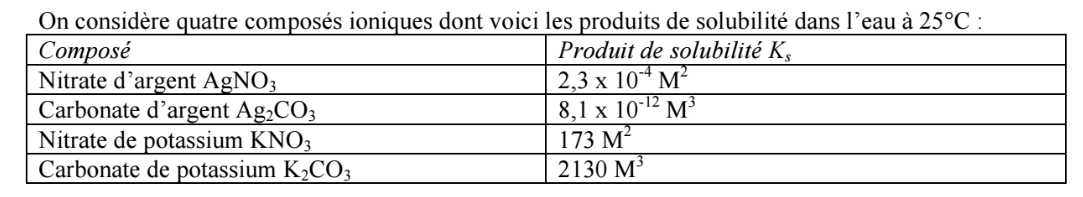
\includegraphics[scale=0.4]{Tab_sol.png}
\end{figure}

\begin{enumerate}
    \item Calculez la solubilité du nitrate d’argent et du carbonate d’argent dans l’eau à $\SI{25}{\celsius}$.
    \item Vous préparez deux solutions à $\ph$ 7 : une solution $\SI{1e-2}{\molar}$ de nitrate d’argent et
une solution $\SI{1e-1}{\molar}$ de carbonate de potassium. Que se passe-t-il si vous
mélangez ces deux solutions à $\SI{25}{\celsius}$ ? Expliquez le phénomène observé.
    \item Sachant que l’acide carbonique $\ce{H2CO3}$ est un acide faible, pensez-vous qu’une modification du $\ph$ du mélange aura un effet sur le phénomène observé ?

Expliquez qualitativement votre réponse et, si possible, exprimez cet effet sous la forme d’une loi mathématique. (NB : le phénomène en question a été illustré dans une vidéo présentée lors d’un cours magistral. Cette vidéo était accessible via un lien cliquable dans le syllabus en ligne).
\end{enumerate}

\textit{Cette question fait actuellement l'objet du cours de chimie et chimie physique 1 (EPL1301).}

\nosolution

\section{( /7)}

L’électrolyse de l’eau en solution acide a également été illustrée par une vidéo. On considère dans ce
cas une cellule électrochimique formée
par deux électrodes plongées dans une
solution acide. Lorsqu’une différence de
potentiel adéquate est appliquée entre les
deux électrodes, la réaction d’électrolyse
se manifeste par l’apparition de bulles
gazeuses d’hydrogène et d’oxygène sur
chacune des électrodes. Répondez aux
questions suivantes en vous servant du
tableau de Nernst ci-contre. Pour rappel,
la constante de Faraday est égale à $\SI{96485}{\coulomb\per\mole}$.

\begin{figure}[h]
    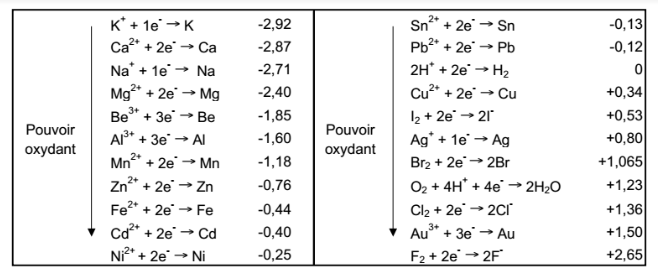
\includegraphics[scale=0.4]{Nernst.png}
    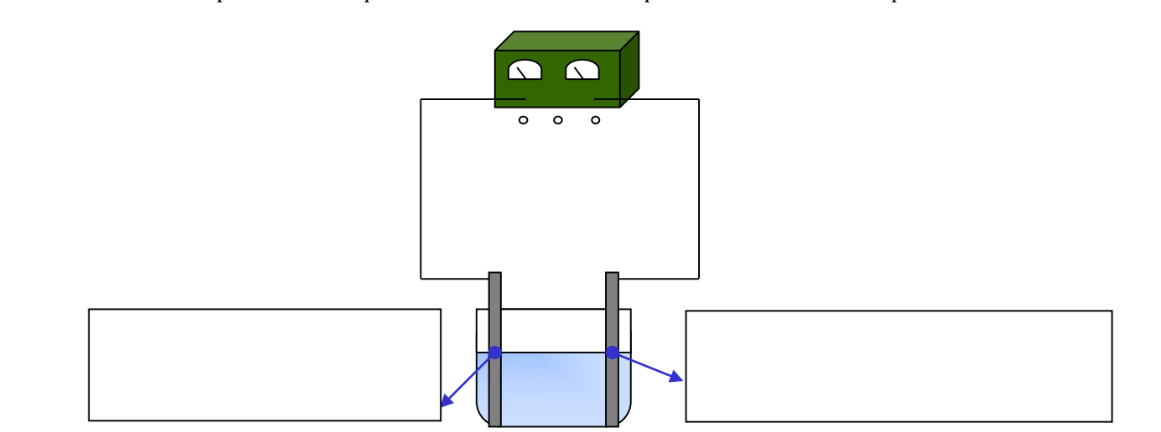
\includegraphics[scale=0.2]{Cellule.png}
\end{figure}

\begin{enumerate}
    \item Décrivez l’expérience d’électrolyse de l’eau en indiquant sur le schéma ci-dessous:
    \begin{itemize}
        \item quelles réactions se déroulent aux deux électrodes,
        \item quelle est l’anode et la cathode,
        \item quelle est la borne positive et la borne négative et quel est le sens de déplacement des
électrons,
        \item quels ions sont présents dans la solution et quel est le sens de leur déplacement.
    \end{itemize}
    \item Donnez la valeur de la tension minimale à appliquer pour induire la réaction d’électrolyse de
l’eau. Discutez le rôle éventuel de la pression appliquée sur la valeur de cette tension.
    \item Discutez l’influence du $\ph$ de la solution sur la valeur de cette tension minimale à appliquer.
Discutez l’avantage éventuel que vous voyez dans l’utilisation d’un $\ph$ faible.
    \item Déduisez de ce qui précède le $\deltr{r} G\std$ de la réaction globale et vérifiez si votre résultat est en accord
avec les données du tableau de valeurs thermodynamiques annexé aux questions d’examen.
    \item (sous-question de bonus : une réponse correcte est susceptible de rapporter des points
supplémentaires s’ajoutant aux points normalement attribués pour l’ensemble de cette question)

Discutez ce qui se passerait si, en plus des cations $\ce{H+}$ (ou $\ce{H3O+}$), la solution contenait des cations $\ce{Cu++}$.
\end{enumerate}

\begin{solution}

\begin{enumerate}
    \item
		La borne positive est à l'anode (électrolyse).
		\begin{solfig}{Electrolyse}{Électrolyse  de l'eau.}
    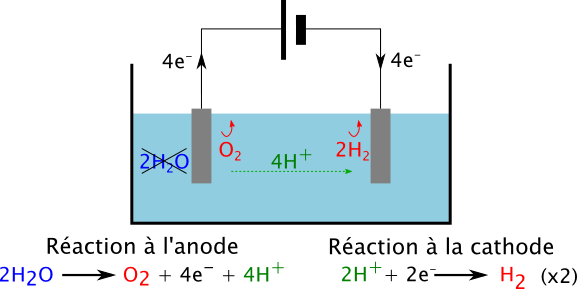
\includegraphics[scale=0.4]{electrolyse.png}
		\end{solfig}

    \item
    $$\phantom{.} E_{\text{cell}} = E_{\text{cathode}} - E_{\text{anode}} = \eca - \ean = \SI{-1.23}{\volt}.$$
    La pression ne fait pas varier la force électromotrice.
    \item Le $\ph$ n'intervient pas dans la tension minimale à appliquer, car celle-ci est constante. Cependant, l'avantage d'un faible $\ph$ est qu'il désigne un concentration élevée d'ions $\ce{H3O+}$, qui facilitent la conduction du courant.
 	\item
    \item Une seconde réaction se déroule à la cathode, la réduction des ions de cuivre:
    $$\phantom{.} \ce{Cu++ +2e- -> Cu} \qquad E\std = \SI{0.34}{\volt}.$$
    La réaction globale est alors:
    $$\phantom{.} \ce{H2O + Cu++ -> (1/2) O2 + 2H+ + Cu} \qquad E\std = \num{0.34} - \num{1.23} = \SI{-0.89}{\volt}.$$
    La force électromotrice de celle-ci est
    $$\phantom{.} E_{\text{cell}}= \num{-0.89} + \frac{RT}{2F}\ln\ce{[Cu^{++}]}.$$
    Cette réaction va donc se faire préférentiellement jusqu'à ce que son potentiel vaille $\SI{-1.23}{\volt}$.
    \begin{align*}
         \num{-0.34} &= \frac{RT}{2F}\ln\ce{[Cu^{++}]} \\
         \implies \ce{[Cu^{++}]} &= \SI{3.16e-12}{\molar}.
    \end{align*}
    Cette concentration étant infime, le potentiel de cette réaction n'atteindra jamais $\SI{-1.23}{\volt}$ et la réaction de réduction des ions $\ce{H+}$ ne se déroulera pas.

\end{enumerate}

\end{solution}

\section{( /10)}

On considère un système fermé gazeux parcourant un cycle moteur réversible composé de 4 transformations :

\begin{itemize}
    \item 1 à 2 : compression adiabatique
    \item 2 à 3 : échauffement isobare
    \item 3 à 4 : détente adiabatique
    \item 4 à 1 : refroidissement isochore
\end{itemize}

Le gaz contenu dans le système est de l’air (gaz parfait) dont les propriétés sont constantes et évaluées à température ambiante.

\begin{enumerate}
    \item
    Le système a été partiellement caractérisé expérimentalement dans un laboratoire. Les valeurs connues sont présentées dans le tableau ci-dessous. On connaît également la quantité de chaleur apportée au système lors de la transformation de 2 à 3 : $Q_{2 \to 3} = \SI{30}{\kilo\joule}$.

À partir des valeurs connues, on vous demande de compléter le tableau ci-dessous en justifiant succinctement vos résultats.
\begin{center}

		\begin{tabular}{|c|c|c|c|c|}

			\hline

			&p$[\si{\bar}]$&$T[\si{\kelvin}]$&$V[\si{\meter\cubed}]$&$S-S_1 [\si{\joule\per\kelvin}]$\\

			\hline

			\num{1} & \num{1} & \num{300} & \num{0.05}&\\

			\hline

			\num{2}&&&&\\

			\hline

			\num{3} & & \num{1700} & &\\

			\hline

               \num{4}&&&&\\

			\hline


		\end{tabular}

	\end{center}
    \item
    Un autre laboratoire a caractérisé un cycle similaire (même succession de transformations, même gaz mais dans des conditions différentes). Dans ce cas, la chaleur apportée au système lors de la transformation 2 à 3 est également connue : $Q_{2 \to 3} = \SI{60}{\kilo\joule}$ de même que le rendement thermique, évalué à \SI{30}{\percent}. Par contre la température $T_3$ n’a pas été mesurée.

On vous demande de compléter le tableau ci-dessous en justifiant succinctement vos résultats.

\begin{center}

		\begin{tabular}{|c|c|c|c|c|}

               &p$[\si{\bar}]$&$T[\si{\kelvin}]$&$V[\si{\meter\cubed}]$&$S-S_1 [\si{\joule\per\kelvin}]$\\

			\hline

			\num{1} & \num{1} & \num{300} & \num{0.05}&\\

			\hline

			\num{2} &&&&\\

			\hline

			\num{3} &&&&\\

			\hline

               \num{4} &&&&\\

			\hline


		\end{tabular}

	\end{center}
\end{enumerate}

\begin{solution}

     \begin{enumerate}
         \item

     Le nombre de moles parcourant le cycle est $\num{2}$ et $\gamma = \frac{C_p}{C_v} = \frac{7/2R}{5/2R} = \num{1.4}$.

     Pour la transformation $2 \to 3$, la chaleur fournie à pression constante équivaut au $\deltr{$2 \to 3$} H$:
     \begin{equation*}
          \phantom{.} \diff H = \diff U + p\diff V + V \diff p = \delta Q + \delta W + p\diff V + V\diff p = \delta Q + V\diff p = \delta Q.
     \end{equation*}
      puisque $\diff p = 0$.
      Ainsi
      $$ \big( \Delta Q \big)_p = \Delta H = C_p \Delta T$$
      $$ \phantom{.} \Delta T = T_3 - T_2 = \frac{Q}{C_p} = \frac{\num{30000}}{\num{2} \cdot 7/2R} = \SI{515.45}{\kelvin}.$$
      On a donc:
      $$\phantom{.} T_2 = T_3 - \num{515.45} = \SI{1184.55}{\kelvin}.$$

      Par la loi de Poisson, on calcule les données sur la 2e ligne.
      \begin{equation*} V_2 = V_1\left(\frac{T_1}{T_2}\right)^{\frac{1}{\gamma - 1}} = \SI{1.614e-3}{\meter\cubed}
      \end{equation*}
      $$ p_2 = p_3 = \frac{nRT_2}{V_2} = \SI{122.05}{\bar}$$
      $$ \phantom{.} V_3 = \frac{nRT_3}{p_3} = \SI{2.31625e-3}{\meter\cubed}.$$
      Par la transformation $4 \to 1$, $V_4 = V_1$.

      Par la loi de Poisson:
      $$T_4 = T_3\left(\frac{V_3}{V_4}\right)^{\gamma - 1} = \SI{497.48}{\kelvin}$$
      $$\phantom{.} p_4 = \frac{nRT_4}{V_4} = \SI{1.6545}{\bar}.$$
      En ce qui concerne les variations d'entropie,
      $$S_2 - S_1 = 0 \qquad \text{(adiabatique)}$$
      $$S_3-S_2=\int_2^3\frac{\delta Q_{2 \to 3}}{T} = \int_2^3 \frac{\diff H}{T} = \int_2^3 \frac{C_p \diff T}{T} = C_p \ln\frac{T_3}{T_2} = \SI{10.513}{\joule\per\kelvin}$$
      $$S_4 - S_3=0 \qquad \text{(adiabatique).}$$
      On obtient donc ce tableau final:
      \begin{center}

     		\begin{tabular}{|c|c|c|c|c|}

     			\hline

     			&p$[\si{\bar}]$&$T[\si{\kelvin}]$&$V[\si{\meter\cubed}]$&$S-S_1 [\si{\joule\per\kelvin}]$\\

     			\hline

     			\num{1}&\num{1}&\num{300}&\num{0.05}&\num{0}\\

     			\hline

     			\num{2}&\num{122}&\num{1184.55}&\num{1.614e-3}&\num{0}\\

     			\hline

     			\num{3}&\num{122}&\num{1700}&\num{2.31625e-3}&\num{10.513}\\

     			\hline

                    \num{4}& \num{1.6545} & \num{497.48}&\num{0.05}&\num{10.513} \\

     			\hline

     		\end{tabular}

     	\end{center}

	\item
	On exprime le rendement:
     \begin{equation*}
          \eta = \frac{\abs{W}}{Q_{\text{h}}} = \frac{Q}{Q_{2 \to 3}} = \frac{Q_{2 \to 3} + Q_{4 \to 1}}{Q_{2 \to 3}} = 1 + \frac{Q_{4 \to 1}}{Q_{2 \to 3}}
     \end{equation*}
	$$ Q_{4 \to 1} = (\eta - 1) Q_{2 \to 3} = (\num{0.3} - \num{1}) \cdot \num{60000} = \SI{-42000}{\joule}$$
	$$Q_{4 \to 1} = \Delta U + W = \Delta U = C_V (T_1 - T_4)$$
	$$\implies T_4 = \frac{-Q_{4 \to 1}}{C_V} + T_1 = \frac{\num{42000}}{\num{2} \cdot \num{5/2}R} + \num{300} = \SI{1310.28}{\kelvin}$$
	$$\phantom{.} p_4 = \frac{nRT_4}{V_4} = \SI{4.35773}{\bar}.$$
	On cherche ensuite $T_3$:
	$$\phantom{,} T_3 = \frac{Q_{2 \to 3}}{C_p} + T_2,$$
	avec
	$$T_2 = T_1 \left(\frac{p_3}{p_1}\right)^{\frac{\gamma - 1}{\gamma}}$$
	et
	$$ \phantom{,} p_3 = p_4 \left(\frac{T_4}{T_3}\right)^{\frac{\gamma}{1-\gamma}},$$
	donc
     \begin{align*}
          T_3 &= \frac{Q_{2 \to 3}}{C_p} + T_1 \left(\frac{p_4}{p_1}\right)^{\frac{\gamma-1}{\gamma}}\left(\frac{T_3}{T_4}\right) \\
          &= \frac{Q_{2 \to 3}}{C_p} \frac{1}{1-\left(\frac{p_4}{p_1}\right)^{\frac{\gamma-1}{\gamma}}\left(\frac{T_1}{T_4}\right)} \\
          &= \SI{1582.72}{\kelvin}.
     \end{align*}
	On en déduit le reste des données:
	$$V_3 = V_4 \left(\frac{T_4}{T_1}\right)^{\frac{1}{\gamma-1}} = \SI{31.18e-3}{\metre\cubed}$$
	$$p_2 = p_3 = \frac{nRT_3}{V_3} = \SI{8,441}{\bar}$$
	$$T_2 = T_3 - \frac{Q_{2 \to 3}}{C_p} = \SI{553.08}{\kelvin}$$
	$$\phantom{.} V_2 = \frac{nRT_2}{p_2} = \SI{10.896e-3}{\metre\cubed}.$$
	Terminons par les variations d'entropie,
	$$\phantom{.} S_3 - S_2 = C_p \ln\frac{T_3}{T_2} = \num{2} \cdot \num{7}/\num{2}R \ln\frac{\num{1582.72}}{\num{553.08}} = \SI{61.2}{\joule\per\kelvin}.$$

	   \begin{center}

		\begin{tabular}{|c|c|c|c|c|}

			\hline

			&p$[\si{\bar}]$&$T[\si{\kelvin}]$&$V[\si{\meter\cubed}]$&$S-S_1 \si{\joule\per\kelvin}$\\

			\hline

			\num{1}&\num{1}&\num{300}&\num{0.05}&\num{0}\\

			\hline

			\num{2}&\num{8.441}&\num{553.08}&\num{10.896e-3}&\num{0}\\

			\hline

			\num{3}&\num{8.441}&\num{1582.72}&\num{31.18e-3}&\num{61.2} \\

			\hline

               \num{4}&\num{4.35773} & \num{1310.28}&\num{0.05}&\num{61.2}\\

			\hline

		\end{tabular}

	\end{center}

	\end{enumerate}

	\end{solution}

	\section{( /10)}

	\begin{enumerate}

	\item L’enthalpie a été définie dans le cadre d’échanges de chaleur à pression constante.

Montrez mathématiquement que, sur base de cette définition et de celle du premier principe, on obtient bien $H = U+pV$.

\item Expliquez mathématiquement et physiquement la présence de l’enthalpie dans
l’expression
$$w_{\text{m}} = -q + \Delta k + g\Delta z + \Delta h$$
\item Établissez rigoureusement le lien mathématique général entre la capacité calorifique à pression constante liée à l’enthalpie et la capacité calorifique à volume constant liée à l’énergie interne.

\item Simplifiez cette relation dans le cas d’un gaz parfait.

\item Expliquez physiquement pourquoi on observe que $C_p > C_V$.

\end{enumerate}

\begin{solution}

\begin{enumerate}
    \item On utilise la notation $\left(Q\right)_p$ pour désigner l'apport de chaleur à pression constante.
    \begin{align*}
         H &= \left(Q\right)_p \\
         \implies \diff H &= \diff \left(Q\right)_p + p\diff V - p\diff V \\
         &= \diff U + p \diff V + V \diff p \qquad (\diff p = 0) \\
         &= \diff U + \diff (pV) \\
         \implies H &= U + pV.
    \end{align*}
    \item Le terme d'enthalpie correspond à
    $$\phantom{,} \Delta U + \Delta (pV),$$
    la somme de la variation de l'énergie interne du système et du travail net d'entrée et de sortie du fluide du système.
    \item
    \textbf{Relation de Mayer}:
    $$\phantom{.} C_p - C_V=\left(\frac{\partial H}{\partial T} \right)_p - \left(\frac{\partial U}{\partial T} \right)_V = \left(\frac{\partial U}{\partial T} \right)_p + \left(\frac{\partial (pV)}{\partial T} \right)_p - \left(\frac{\partial U}{\partial T} \right)_V.$$

    \item
    En simplifiant les deux dérivées partielles de l’énergie interne puisqu’elles sont égales (car l’énergie est uniquement fonction de la température et pas de la pression ou du volume), on obtient
$$\phantom{.} C_p - C_V=\left(\frac{\partial (pV)}{\partial T} \right)_p = \left(\frac{\partial (nRT)}{\partial T} \right)_p = nR.$$

    \item
    La capacité calorifique à volume constant est une mesure de la quantité de chaleur à apporter à un système maintenu à volume constant pour en augmenter la température d’un degré.

    La capacité calorifique à pression constante est une mesure de la quantité de chaleur à apporter à un système maintenu à pression constante pour en augmenter la température d’un degré.

    La différence reflète l’apport supplémentaire de chaleur à fournir pour compenser le travail effectué dans le cas à pression constante.
\end{enumerate}

\end{solution}

\end{document}
